
\documentclass[preprint,12pt]{elsarticle}

\usepackage[spanish]{babel}
\usepackage{amssymb}
\usepackage{graphicx}
\usepackage{lineno}
\usepackage[utf8]{inputenc}
\usepackage{url}
\usepackage{natbib} 
\usepackage{amsmath} 
\usepackage{amssymb} 

\begin{document}
	
	\begin{frontmatter} 

		\title{\huge MÁQUINAS VIRTUALES VS CONTENEDORES}
		
		\author{Estrella Palacios, Katherine Lizbeth              	(2016056193))}
		\author{Gonzales Cave, Angel Gabriel              	        (2017057861))}
		\author{Porlles Carrillo, Diego Armando	         	(XXXXXXXXXX))} %CAMBIAR CODIGO 
		\author{Quispe Mamani, José Luis             		(2015053235))} %CAMBIAR CODIGO 
		\address{Escuela Profesional de Ingeniería de Sistemas}
		\address{Universidad Privada de Tacna}
		\address{Tacna, Perú}
		
%% ABSTRACT --------------------------------------------------------------------------------------------------------------------

		\begin{abstract}
		


		\end{abstract}

%% ----------------------------------------------------------------------------------------------------------------------------------

	\end{frontmatter}

%% RESUMEN ---------------------------------------------------------------------------------------------------------------------

\section{Resumen}



%% ----------------------------------------------------------------------------------------------------------------------------------


%% INTRODUCION ----------------------------------------------------------------------------------------------------------------

\section{Introducción}

La mayoría de empresas utilizan múltiples servidores para llevar a cabo sus operaciones, y para la continuidad de sus operaciones tienen dos o mas servidores ejecutando los mismos servicios en diferentes servidores .Esto se debe a que no se puede garantizar que un sistema operativo funcione correctamente todos los días durante el año. Por esta razón cada servicio se separa y se deja funcionando en un host distinto, pero esta solución resulta costosa y difícil de administrar por el número de máquinas y el espacio requerido para su funcionamiento.
Debido a esta problema surgieron las máquinas virtuales que permiten la ejecución de múltiples sistemas operativos llamados invitados en una sola máquina física llamada anfitrón.  



%% ----------------------------------------------------------------------------------------------------------------------------------


%% MARCO TEÓRICO ------------------------------------------------------------------------------------------------------------

\section{Marco Teórico}

%% PRIMERA SUBSECCION 

\subsection {\textbf{Máquina Virtual}}
Una máquina virtual (VM) es una computadora compuesta completamente de software que puede ejecutar su propio sistema operativo y aplicaciones como si fuera una computadora física. Una VM se comporta exactamente como una computadora física y contiene su propia CPU virtual (basada en software), RAM, disco duro y tarjeta de interfaz de red (NIC).\cite{Citrix2018}


\subsection {\textbf{Hyper-V}}
Hyper-V es un hipervisor que permite la virtualización de diferentes sistemas operativos, que se ejecutan al mismo tiempo sobre un sistema físico, sin que se vean interferidos entre ellos. Esta separación de entornos se consigue mediante la creación de una capa de abstracción entre el hardware de la máquina física (también conocida como host) y el sistema operativo que se ejecuta dentro del entorno virtualizado (también conocido como máquina virtual o huésped). De este modo, los diferentes recursos de la máquina física (tarjeta de red, memoria RAM, etc.) se dividen y se reparten entre uno o más entornos virtualizados.

\begin{figure}[htb]
	\begin{center}
		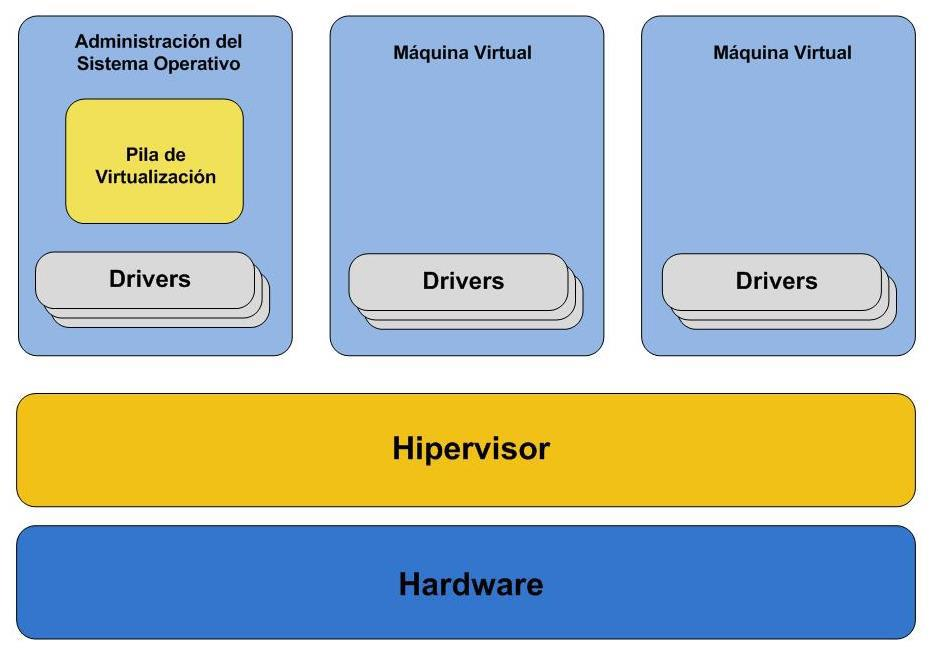
\includegraphics[width=10cm]{./IMAGENES/Hyper-v} 
		\caption{Hipervisor}
	\end{center}
\end{figure}
El hipervisor, constituye una pequeña capa de software entre el hardware y los diferentes sistemas operativos instalados en el sistema. Es el encargado de ejecutar múltiples instancias de sistemas operativos de forma aislada a través del uso de múltiples instancias de ejecución conocidas como particiones.

El hipervisor se divide en dos capas diferentes. La capa inferior, corresponde a la implementación de un microkernel que soporta acceso a memoria, uso de hilos, uso de señales y un mecanismo de abstracción del hardware; mientras que la capa superior, se encarga de proporcionar los servicios de virtualización.\cite{Hyperv2019}

\subsubsection{\textbf{Beneficios}}
La virtualización realizada por Hyper-V, proporciona diferentes beneficios tanto técnicos como de gestión, que
se detallan a continuación:
\begin{itemize}
\item Mayor eficiencia de los recursos de la máquina física.
\item Reducción de los costes de operación y mantenimiento de la máquina física.
\item Reducción del tiempo requerido para el despliegue y configuración del hardware y software, así como la
realización de las pruebas correspondientes al entorno físico sobre el que se despliega el servicio Hyper-V.
\item Los recursos físicos son gestionados por Hyper-V para proporcionar entornos totalmente aislados.
\item Implementación de entornos de escritorios virtuales a través de VDI.
\item Posibilidad de crear entornos de testing o prueba sin que sea necesario obtener equipamiento hardware
\end{itemize}
\cite{Hyperv2019}

\subsubsection{\textbf{Limitaciones}}
El servicio Hyper-V posee una serie de limitaciones en cuanto a la cantidad de recursos que puede utilizar. Del
mismo modo, cada una de las máquinas virtuales gestionadas por el servicio de virtualización posee una serie de
limitaciones con respecto a sus recursos de tipo físico asignados.
Las limitaciones del servicio Hyper-V son las siguientes:
\begin{itemize}
\item Número de procesadores lógicos, 512.
\item Procesadores virtuales por cada procesador lógico, sin limitación.
\item Máquinas virtuales en ejecución por servidor, 1024.
\item Procesadores virtuales por servidor, 2048.
\item Memoria RAM, 24 TB.
\item Capacidad de almacenamiento, sin limitación. Depende de la capacidad de almacenamiento del sistema
operativo base.
\item Redes de área de almacenamiento (SAN) virtuales, sin limitación.
\item Adaptadores de red físicos, sin limitación.
\item Equipos de adaptadores de red (NIC Teaming), sin limitación.
\item Redes virtuales (conmutadores virtuales), sin limitación. Depende de los recursos del sistema físico.
\item Puertos de los conmutadores de red virtuales por servidor, sin limitación. Depende de los recursos del sistema físico.
\end{itemize}
\cite{Hyperv2019}

\subsubsection{\textbf{Componentes Físicos Virtualizados}}
El servicio Hyper-V se encarga de virtualizar los recursos físicos de los que dispone en la máquina que despliega
el servicio de virtualización.
Los recursos virtualizados por el servicio se indican a continuación:
\begin{itemize}
\item Procesadores virtuales.
\item Memoria RAM.
\item Discos duros virtuales.
\item Adaptadores de red virtuales.
\item Unidades de CD/DVD virtuales.
\item Unidades de disquete virtuales.
\item Adaptadores de video virtuales.
\item Dispositivos de entrada de datos (ratón y teclado) virtuales.
\end{itemize}
\cite{Hyperv2019}

\subsection {\textbf{XenServer}}
XenServer es la plataforma completa de virtualización de servidores de Citrix. XenServer está optimizado para servidores virtuales Windows y Linux.

XenServer se ejecuta directamente en el hardware del servidor sin requerir un sistema operativo subyacente, lo que resulta en un sistema eficiente y escalable. XenServer funciona abstrayendo elementos de la máquina física (como discos duros, recursos y puertos) y asignándolos a las máquinas virtuales que se ejecutan en él.

Usar XenServer reduce los costos :
\begin{itemize}
\item Consolidación de múltiples máquinas virtuales en servidores físicos
\end{itemize}
Usar XenServer aumenta la flexibilidad al:
\begin{itemize}
\item Aumento de la disponibilidad de máquinas virtuales mediante el uso de alta disponibilidad para configurar políticas que reinicien máquinas virtuales en otro host XenServer si falla uno.
\item Mayor portabilidad de las imágenes de VM, ya que una imagen de VM funcionará en una variedad de infraestructuras de implementación
\end{itemize}

\subsubsection{\textbf{vApps}}
Una vApp es un grupo lógico de una o más máquinas virtuales (VM) relacionadas que se pueden iniciar como una sola entidad en caso de un desastre. Cuando se inicia una vApp, las máquinas virtuales contenidas en la vApp comenzarán en un orden predefinido por el usuario, para permitir que las máquinas virtuales que dependen unas de otras se secuencian automáticamente. Esto significa que un administrador ya no tiene que secuenciar manualmente el inicio de máquinas virtuales dependientes si un servicio completo requiere reiniciar.  La funcionalidad de vApp es particularmente útil en la situación de recuperación de desastres donde un administrador puede elegir agrupar todas las máquinas virtuales que residen en el mismo repositorio de almacenamiento.

\subsubsection{\textbf{Monitoreo y Gestión XenServer}}
XenServer proporciona un monitoreo detallado de las métricas de rendimiento, incluida la CPU, la memoria, el disco, la red  y el almacenamiento para cada máquina virtual.
XenServer también proporciona alertas de sistema y rendimiento. Las alertas son notificaciones que se producen en respuesta a eventos seleccionados del sistema, o cuando la CPU, el uso de memoria, la red, el rendimiento de almacenamiento o la actividad del disco de la VM superan un umbral especificado en un host, VM o repositorio de almacenamiento administrado.\cite{Citrix2018}

%%Ejemplo de cita
\cite{Gartner} 

\begin{itemize}
	\item x
	\item y
	\item z
\end{itemize}

\subsubsection{\textbf{A2}}

EDITAR\\

\subsubsection{\textbf{A3}}

EDITAR\\


%% SEGUNDA SUBSECCION

\subsection{\textbf{B}}

\subsubsection{\textbf{B1}}

EDITAR\\

%% Ejemplo de inclusión de imagen
\begin{figure}[htb]
	\begin{center}
		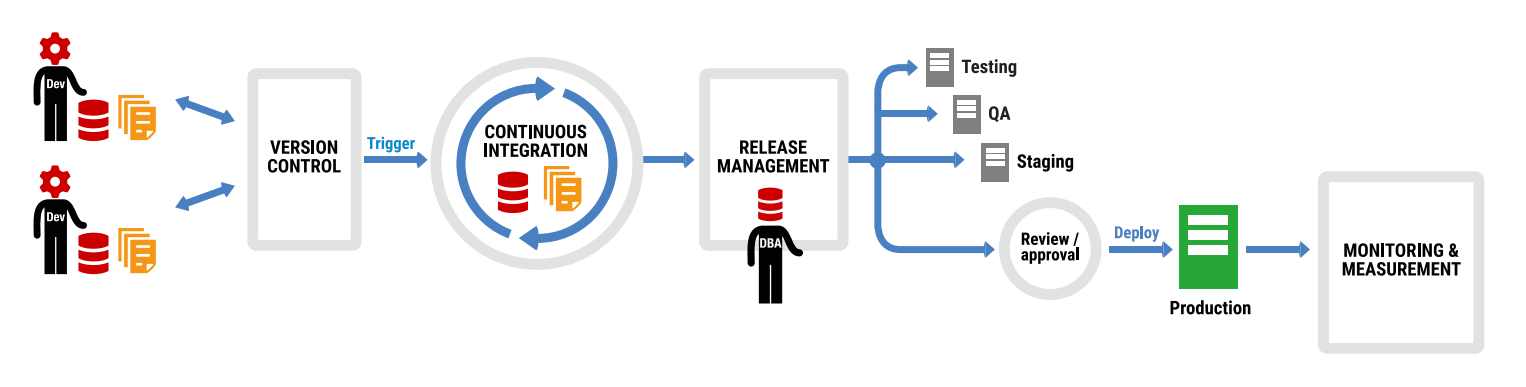
\includegraphics[width=14cm]{./IMAGENES/basededatos_1} 
		\caption{Incluyendo la base de datos en DevOps}
	\end{center}
\end{figure}

\subsubsection{\textbf{B2}}

EDITAR\\

%% TERCERA SUBSECCION
\subsection{\textbf{Contenedores}}
Para las tecnologías de la información, es bien sabido que de nada sirve un Servidor de Cómputo (equipo de cómputo físico o virtual, que permite ofrecer aplicaciones específicas a Usuarios finales), sin la piedra angular de la Infraestructura. En estos equipos es posible, tras la instalación de un robusto, seguro y escalable Sistema Operativo (como Red Hat Enterprise Linux), aprovisionar aplicaciones capaces de atender las peticiones de un Usuario, para subsanar cualquier necesidad informática. Servidores de Correo Electrónico, servidores de Páginas Web (HTTP Servers), servidores de Aplicaciones (como Red Hat JBoss Application Server), etc.

Si bien las máquinas virtuales (VM) tradicionales permiten la virtualización de la infraestructura de computación, los contenedores habilitan la de las aplicaciones de software. A diferencia de las máquinas virtuales, los contenedores utilizan el sistema operativo (SO) de su host en lugar de proporcionar uno propio.

¿Qué es lo que se viene a la mente cuando mencionamos la palabra "Contenedor"? Obviamente que esas inmensas cajas metálicas que, apiladas por cientos sobre buques plataforma, nos permiten trasladar de manera segura cualquier mercancía o bien usando los bastos océanos de nuestro planeta. Baste decir sólo como referencia, que aproximadamente el 95 por ciento de los bienes que se producen en cualquier país del mundo, son trasladados (exportados-importados) usando contenedores, buques plataforma y los océanos.

\subsubsection{\textbf(¿Por qué utilizar contenedores?)}}
Dado que no incluyen sistemas operativos completos, los contenedores requieren recursos informáticos mínimos y son rápidos y fáciles de instalar. Esta eficiencia permite que se implementen en clústeres, con contenedores individuales que encapsulan componentes únicos de aplicaciones complejas. Separar los componentes de la aplicación en diferentes contenedores permite a los desarrolladores actualizar componentes individuales sin necesidad de rehacer la aplicación completa.

De manera muy semejante, los Contenedores Informáticos utilizan una pieza de software a modo de un buque plataforma (ese software casi siempre es Docker), aprovechando ese océano de recursos informáticos (procesador, memoria, red y almacenamiento) sobre el mismo Sistema Operativo.

\begin{itemize}

\item x
\item y
\item z

\end{itemize}
\subsubsection{\textbf{¿Qué es lo que dice Docker?}}
"Una imagen de contenedor es un paquete ligero, independiente, ejecutable de una pieza de software que incluye todo lo necesario para ejecutarlo: código, tiempo de ejecución, herramientas del sistema, bibliotecas del sistema, configuraciones."

Vale la pena agregar que: "Disponible para aplicaciones basadas en Linux, el software en contenedor siempre funcionará igual, independientemente del entorno." Como ya lo habíamos mencionado líneas arriba: "Los contenedores aíslan el software de su entorno, por ejemplo, las diferencias entre los entornos de desarrollo y de etapas, y ayudan a reducir los conflictos entre los equipos que ejecutan software diferente en la misma infraestructura."

Ahora bien. ¿Qué es Docker? Es proyecto de código abierto que automatiza el despliegue de aplicaciones dentro de contenedores de software, proporcionando una capa adicional de abstracción y automatización de Virtualización a nivel de sistema operativo en Linux.


%% ----------------------------------------------------------------------------------------------------------------------------------
 


%% ANÁLISIS ( APLICACIÓN ) ---------------------------------------------------------------------------------------------------

\section{Análisis}

\subsection{\textbf{Análisis 1}}
EDITAR\\

\subsection{\textbf{Análisis 2}}
EDITAR\\

\subsection{\textbf{¿Por qué Contenedores y no Máquinas Virtuales?}}
Sólo para comenzar, los Contenedores son más ligeros, requieren de menos recursos informáticos y por ende más versátiles. Al igual que las Máquinas Virtuales, ofrecen portabilidad, escalabilidad y son tan seguros como lo es el Sistema Operativo donde se están ejecutando. Lo que hace a los Contenedores, para ciertas ocasiones, no muy adecuados, es para esos escenarios en loa que se requieren Sistemas Operativos de distinta versión (sobre todo versión de Kernel), pues el requisito indispensable para que puedan ejecutarse los contenedores en el mismo servidor físico, es precisamente que todas éstas puedan ejecutarse sobre la misma versión del Kernel.

Los Contenedores aíslan las aplicaciones entre sí, a menos que se les conecte explícitamente. Eso significa que no existen dependencias conflictivas o contención de recursos, se establecen límites de recursos explícitos para cada servicio. Es importante destacar que se trata de una capa adicional de seguridad ya que sus aplicaciones no se ejecutan directamente en el sistema operativo host.

\subsection{\textbf{¿Cómo podemos ofrecer una solución segura, confiable, escalable y completa de Contenedores con Software Red Hat?}}
Infraestructura con Red Hat Enterprise Linux: Manténgase ligero y ejecute sus contenedores Linux con un sistema operativo optimizado, seguro y de mínima huella. Platadorma con Red Hat Open Shift: Desarrolle, implemente y administre sus contenedores en cualquier lugar, a cualquier escala. Red Hat® OpenShift es una plataforma de aplicaciones de contenedores que incluye Docker y Kubernetes. Independientemente de la arquitectura de sus aplicaciones, OpenShift le permite construir, desarrollar e implementar fácil y rápidamente en casi cualquier infraestructura, pública o privada

%% ----------------------------------------------------------------------------------------------------------------------------------


%% CONCLUSIONES ---------------------------------------------------------------------------------------------------------------

\section{Conclusiones}

\begin{itemize}

\item Conclusion 1 : \\

\item Conclusion 2 : \\ 

\item Conclusion 3 : \\ 

\item Conclusion 4 : \\ 
\end{itemize}

%% ----------------------------------------------------------------------------------------------------------------------------------

%%  REFERENCIAS BIBLIOGRÁFICAS ------------------------------------------------------------------------------------------
	
	\newpage
	
	\bibliographystyle{apalike} 	%ESTILO
	\bibliography{BIBLIOGRAFIA}	 
	
	
\end{document}
